%Die Angabe des schlauen Spruchs auf diesem Wege funtioniert nur,
%wenn keine Änderung des Kapitels mittels den in preambel/chapterheads.tex
%vorgeschlagenen Möglichkeiten durchgeführt wurde.
%\setchapterpreamble[u]{%
%\dictum[Albert Einstein]{Probleme kann man niemals mit derselben Denkweise lösen, durch die sie entstanden sind.}
%}

\chapter{Ergebnisse und Resultate}
\label{chap:results}

Im nachfolgenden Kapitel werden die Einflüsse der entwickelten Erweiterungen evaluiert und mit dem Standard-Verfahren von Debevec und Malik verglichen (siehe \autoref{fig:res:1}). Für die Experimente werden die Belichtungsserien u.a. mit additivem Gauss-Rauschen und \gls{SaltAndPepperNoise} modifiziert, um das Verhalten der Erweiterungen unter diesen Einflüssen analysieren zu können.


\begin{figure}
  \begin{center}
        \begin{overpic}[width=0.48\textwidth]{results/E1}
                \put(-0,0){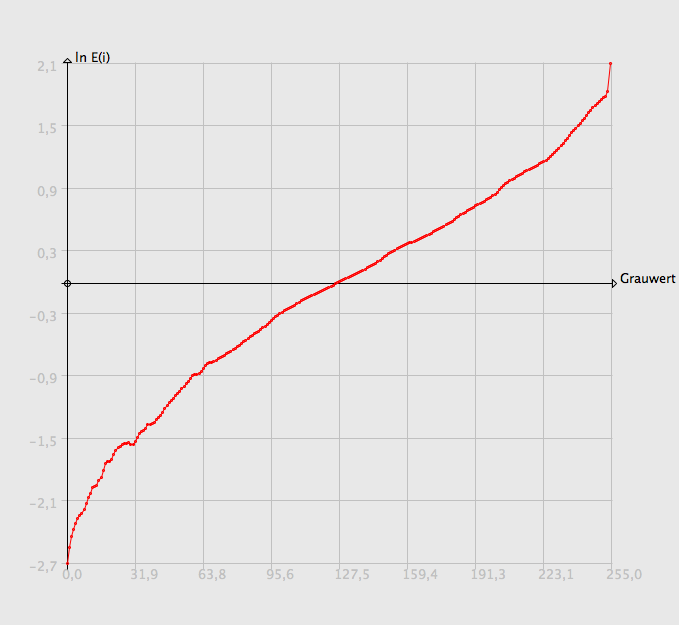
\includegraphics[width=3cm]{results/g1}}
        \end{overpic}
        \hfill
        \begin{overpic}[width=0.48\textwidth]{results/E1_external}
            \put(-0,0){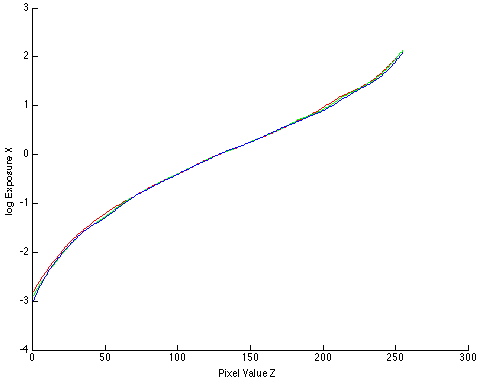
\includegraphics[width=3cm]{results/g1_external}}
        \end{overpic}
    \caption{\textit{Berechnung der Antwortkurve (inkl. Resultat)} --- \textbf{links:} Mit den hier vorgestellten Erweiterungen, \textbf{rechts:} Herkömmliche Implementierung (hier von Mathias Eitz, siehe \autoref{sec:implementations})}
    \label{fig:res:1}
  \end{center}
\end{figure}

Dazu werden folgende Symbole mit den angegebenen Standardwerten (falls nicht anders angegeben) verwendet:
\begin{description}
\item[$\lambda$]: Gewicht des Glattheitsterms für $\b g$, Standard: $50$
\item[$\mu$]: Gewicht der Monotonie-Beschränkung für $\b g$, Standard: $0$
\item[$\alpha$]: Gewicht der räumlichen Glattheit für $\b E$, Standard: $0$
\item[$\#$]: Anzahl der Iterationen beim iterativen Lösen, Standard: $10$
\item[$\sigma$]: Standardabweichung des additiven Gauss-Rauschen, Standard: $0$

\end{description}

Um die Bilder einheitlich zu vergleichen, wurde bei allen Resultaten der globale \gls{Tone-Mapping}-Operator von Reinhard (siehe \autoref{sub:tone:global}, \cite{ReinhardToneMapper}) verwendet. Außerdem wurde für nahezu alle Vergleiche die gleiche Belichtungsserie (siehe \autoref{fig:picture-serie}) verwendet, welche bereits registriert ist \cite{tellone}.



\section{Ergebnisse mit Monotonie-Bedingung}
Im ersten durchgeführten Experiment wurde der Einfluss der Monotonie-Bedingung auf die Antwortkurve $\b g$ untersucht.
Bei den meisten Bildern ist diese bereits von sich aus monoton steigend, obwohl es nicht durch das Standard-Verfahren gefordert ist. Um eine Bildserie zu erhalten, bei der die Kurve diese Eigenschaft nicht bereits durch das Standard-Verfahren erhält, wurden eigene Bilder aufgenommen (siehe \autoref{fig:mon:1}). Diese Belichtungsserie liefert zunächst eine recht unförmige Antwortkurve, welche auch durch mehr Iterationen nicht weiter konvergiert. Durch die Erweiterung der Monotonie kann die Kurve entsprechend begradigt und verbessert werden. Es fällt auf, dass Überschwinger in diesem Beispiel durch die Monotonie-Bedingung quasi abgesägt werden. 

\begin{figure}
  \begin{center}
    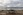
\includegraphics[height=3.5cm]{sample_2/1}
    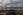
\includegraphics[height=3.5cm]{sample_2/2}
    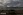
\includegraphics[height=3.5cm]{sample_2/3}
     \hfill
    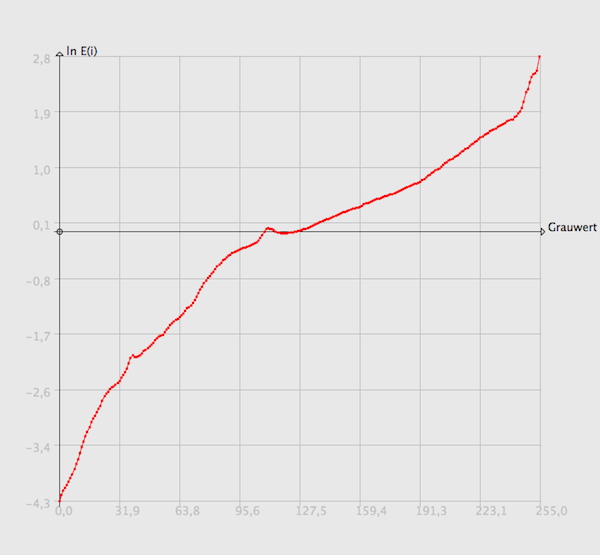
\includegraphics[height=3.5cm]{sample_2/g_no_mon}
    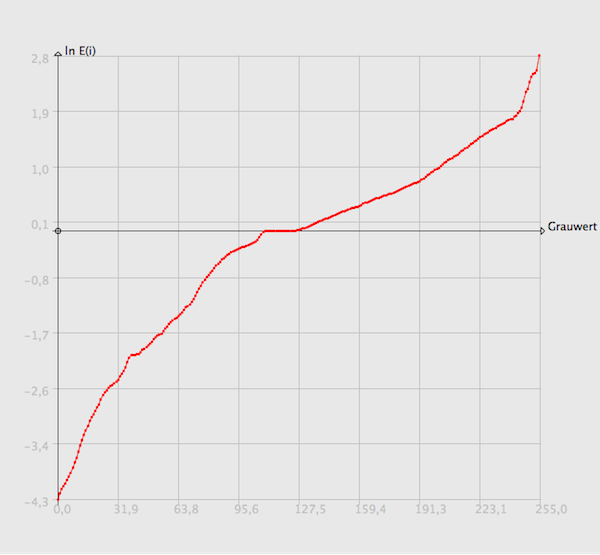
\includegraphics[height=3.5cm]{sample_2/g_mon}
    \caption{\textit{Monotonie-Forderung} --- Belichtungsserie (Belichtungszeiten: $\frac{1}{8000}$, $\frac{1}{640}$, $\frac{1}{100}$),  Antwortkurve ohne Monotonie-Forderung, Antwortkurve mit Monotonie-Forderung  (v.l.n.r.)}
    \label{fig:mon:1}
  \end{center}
\end{figure}



\section{Ergebnisse mit räumlichem Glattheitsterm}

\begin{figure}[b]
  \begin{center}
    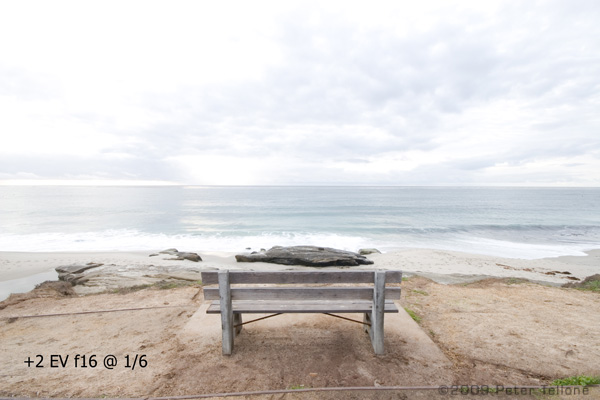
\includegraphics[width=2cm]{img/1_6}
    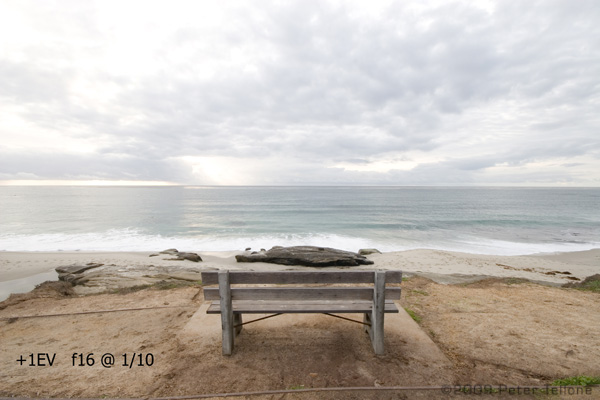
\includegraphics[width=2cm]{img/1_10}
    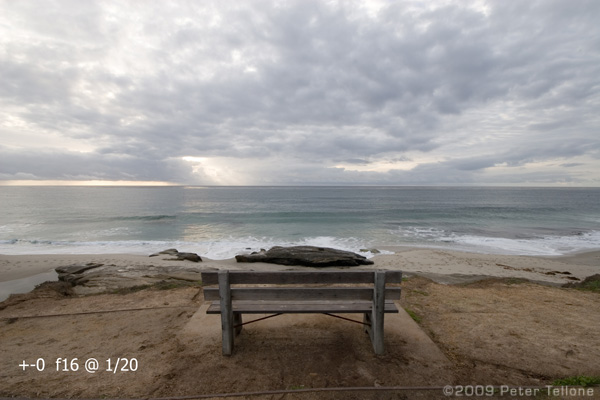
\includegraphics[width=2cm]{img/1_20}
    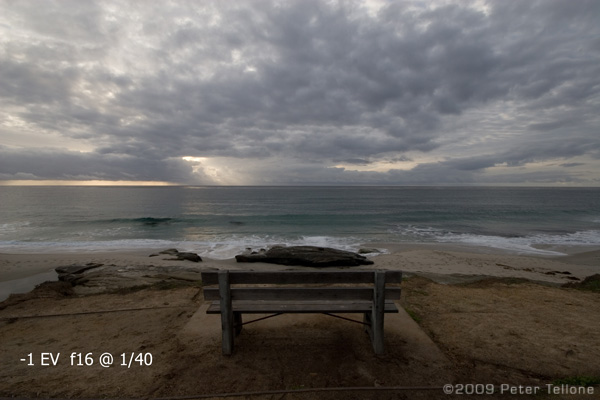
\includegraphics[width=2cm]{img/1_40}
    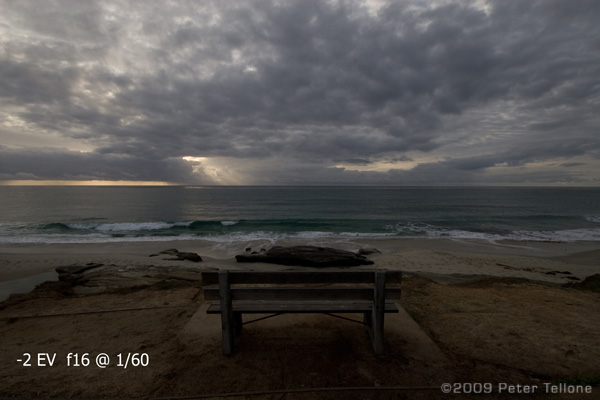
\includegraphics[width=2cm]{img/1_60}
    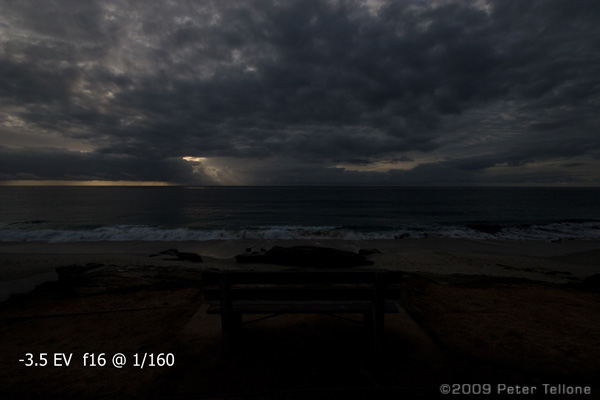
\includegraphics[width=2cm]{img/1_160}
    \caption{\textit{Verwendete Belichtungsserie} --- Sechs Einzelaufnahmen mit den Belichtungszeiten $\frac{1}{6}, \frac{1}{10}, \frac{1}{20}, \frac{1}{40}, \frac{1}{60}\mbox{ und }\frac{1}{160}$ (v.l.n.r) \cite{tellone}}
    \label{fig:picture-serie}
  \end{center}
\end{figure}

Im zweiten Experiment wurde der Einfluss des räumlichen Glattheitsterm auf die Standard-Belichtungsserie (siehe \autoref{fig:picture-serie}) untersucht.

Die Erweiterung des räumlichen Glattheitsterms sorgt dafür, dass die benachbarten Pixel bei der Berechnung der \gls{Radiance Map} berücksichtigt werden. Wie in \autoref{fig:raum:1} zu sehen, hat dies insbesondere bei Messfehlern (hier 4\% \gls{SaltAndPepperNoise}) einen enormen Vorteil gegenüber dem herkömmlichen Verfahren.

\gls{SaltAndPepperNoise} ist eine besonder Form von Rauschen, bei dem einzelne Bildpunkte zufällig weiß oder schwarz werden. Die Prozent-Angabe in diesem Zusammenhang gibt an, welche Menge an Pixeln davon betroffen sein kann.

Auch durch Störungen -- wie das additive Gauss-Rauschen ($\sigma=10$, siehe \autoref{fig:raum:2}) -- sind die Ergebnisse schärfer und das Rauschen auf den Eingangsbildern wird reduziert.


\begin{figure}
  \begin{center}
    \begin{tikzpicture}[spy using outlines={circle,red,magnification=3,size=4cm, connect spies}]
        \node {
            \begin{overpic}[width=0.5\textwidth]{raum/E_ohne}
                \put(-0,0){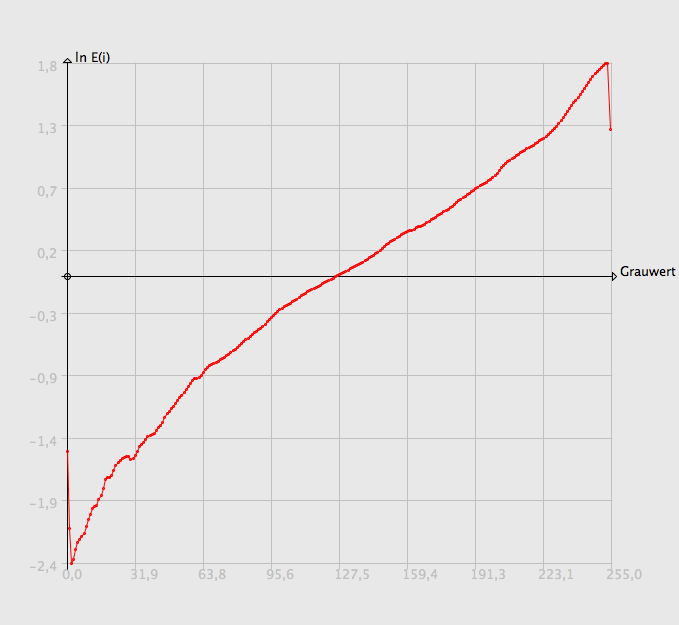
\includegraphics[width=3cm]{raum/g_ohne}}
            \end{overpic}
        };
        \spy on (1.4,-1.3) in node [left] at (9.5,0);
    \end{tikzpicture}
    
    \begin{tikzpicture}[spy using outlines={circle,red,magnification=3,size=4cm, connect spies}]
        \node {
            \begin{overpic}[width=0.5\textwidth]{raum/E_mit}
                \put(-0,0){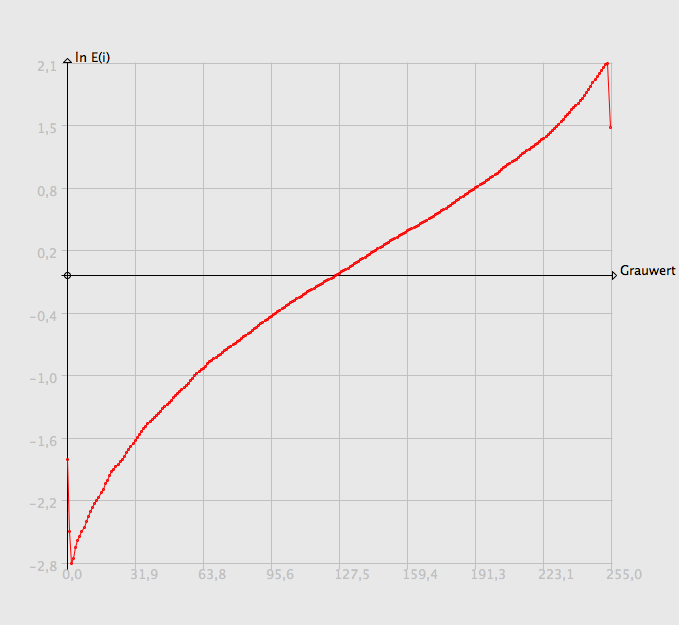
\includegraphics[width=3cm]{raum/g_mit}}
            \end{overpic}
        };
        \spy on (1.4,-1.3) in node [left] at (9.5,0);
    \end{tikzpicture}
    \caption{\textit{Räumlicher Glattheitsterm (mit 4\% \gls{SaltAndPepperNoise})} --- \textbf{oben:} Antwortkurve und zugehöriges HDR Bild ohne räumlichen Glattheitsterm, \textbf{unten:} Antwortkurve mit räumlichem Glattheitsterm ($\alpha = 1$) und zugehöriges HDR-Bild. Das \gls{SaltAndPepperNoise} ist im unteren Bild quasi nicht mehr zu erkennen.}
    \label{fig:raum:1}
  \end{center}
\end{figure}

\begin{figure}
  \begin{center}
    \begin{tikzpicture}[spy using outlines={circle,red,magnification=3,size=4cm, connect spies}]
        \node {
            \begin{overpic}[width=0.5\textwidth]{raum/E_gauss_ohne}
                \put(-0,0){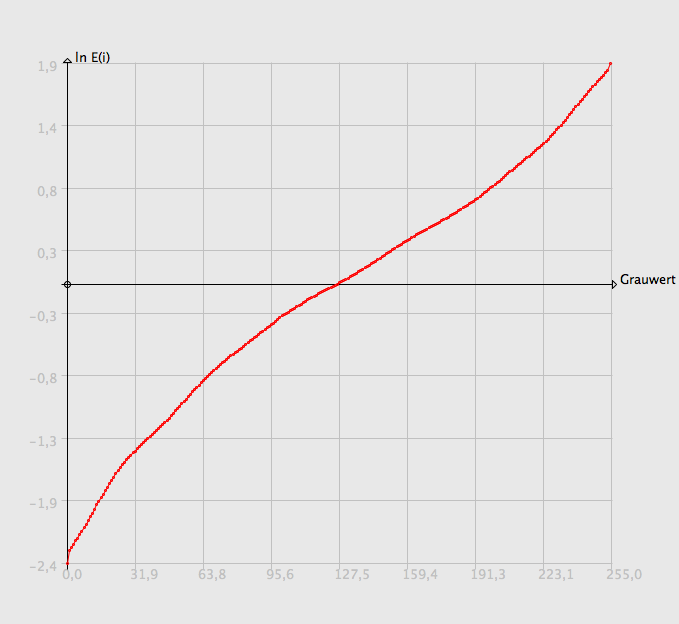
\includegraphics[width=3cm]{raum/g_gauss_ohne}}
            \end{overpic}
        };
        \spy on (1.4,-1.3) in node [left] at (9.5,0);
    \end{tikzpicture}
    
    \begin{tikzpicture}[spy using outlines={circle,red,magnification=3,size=4cm, connect spies}]
        \node {
            \begin{overpic}[width=0.5\textwidth]{raum/E_gauss_mit}
                \put(-0,0){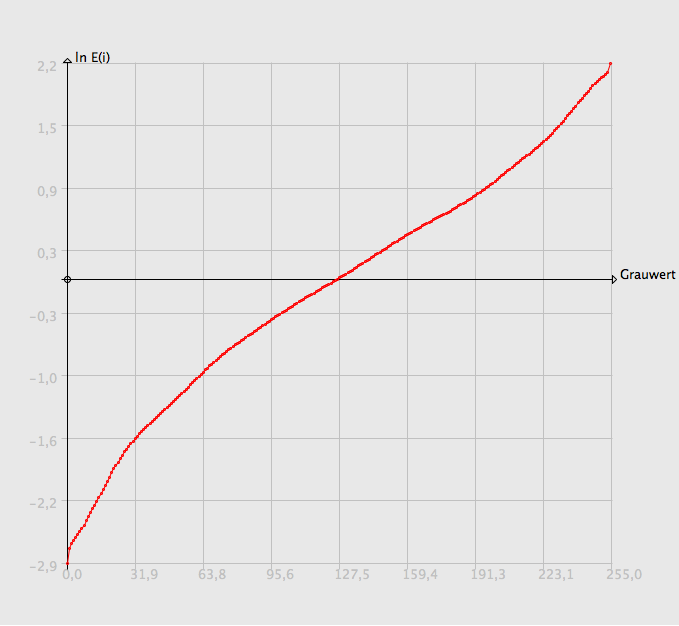
\includegraphics[width=3cm]{raum/g_gauss_mit}}
            \end{overpic}
        };
        \spy on (1.4,-1.3) in node [left] at (9.5,0);
    \end{tikzpicture}
    \caption{\textit{Räumlicher Glattheitsterm (mit additivem Gauss-Rauschen $\sigma = 10$)} --- \textbf{oben:} Antwortkurve und zugehöriges HDR Bild ohne räumlichen Glattheitsterm, \textbf{unten:} Antwortkurve mit räumlichem Glattheitsterm ($\alpha = 1$) und zugehöriges HDR-Bild.}
    \label{fig:raum:2}
  \end{center}
\end{figure}

\section{Ergebnisse mit subquadratischen Bestrafungstermen}

Im dritten Experiment wurde zunächst der Einfluss der subquadratischen Bestrafungsterme unter Standard-Bedingungen getestet. Unter normalen Umständen liefert das Verfahren kaum eine Verbesserung der Ausgabe (siehe \autoref{fig:robust:1}). Lediglich der Kontrast und die Konturenschärfe im \gls{HDR}-Bild sind etwas verbessert. 

In einem darauf aufbauendem Experiment wurde nun auch noch Rauschen (hier \gls{SaltAndPepperNoise}, siehe \autoref{fig:robust:2}) simuliert. Dieses Störsignal konnte durch den Einsatz der subquadratischen Bestrafungsterme erfolgreich reduziert werden, sodass dieses im Ausgabebild nicht mehr zu erkennen ist. Der Effekt entsteht durch die geringere Gewichtung der Ausreißer bei der Berechnung von $\b g$ und $\b E$.


Von der Erweiterung des räumlichen Glattheitsterms um robuste Funktionen wurde eine Verbesserung der Kantenerhaltung erwartet. Diese Erwartung wurde jedoch, wie in \autoref{fig:robust:kanten} zu erkennen ist, nicht erfüllt. Die Verbesserungen sind trotz hoher Gewichtung so minimal, dass sie kaum zu erkennen sind.


\begin{figure}
  \begin{center}
    \begin{tikzpicture}[spy using outlines={circle,red,magnification=3,size=4cm, connect spies}]
        \node {
            \begin{overpic}[width=0.5\textwidth]{results/E1}
                \put(-0,0){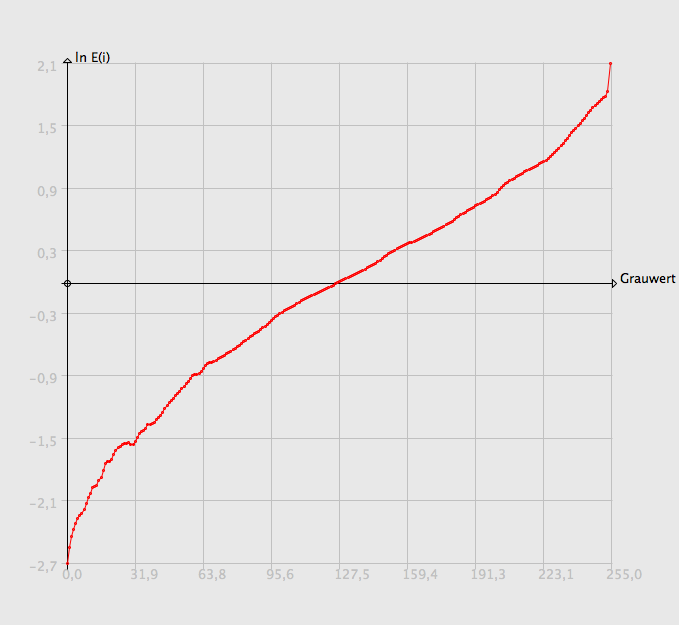
\includegraphics[width=3cm]{results/g1}}
            \end{overpic}
        };
        \spy on (1.4,-1.3) in node [left] at (9.5,0);
    \end{tikzpicture}
    
    \begin{tikzpicture}[spy using outlines={circle,red,magnification=3,size=4cm, connect spies}]
        \node {
            \begin{overpic}[width=0.5\textwidth]{robust/E_mit_robust}
                \put(-0,0){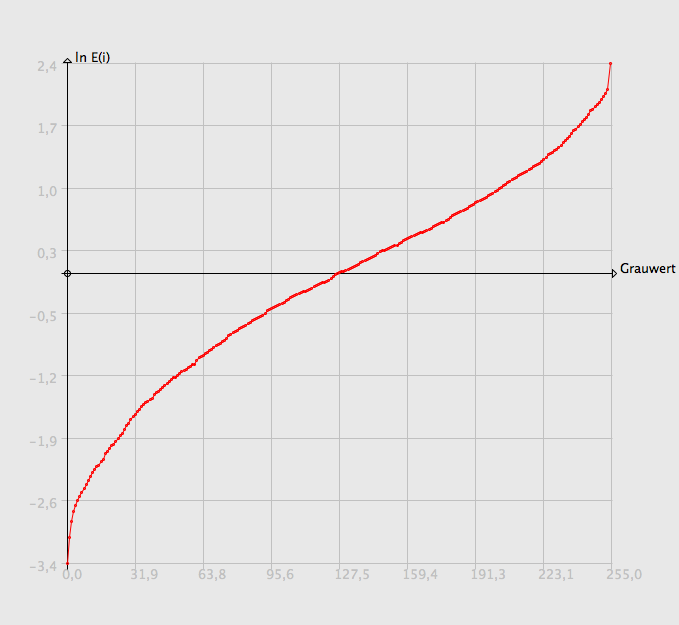
\includegraphics[width=3cm]{robust/g_mit_robust}}
            \end{overpic}
        };
        \spy on (1.4,-1.3) in node [left] at (9.5,0);
    \end{tikzpicture}
    \caption{\textit{Subquadratischen Bestrafungsfunktionen} --- \textbf{oben:} Standardverfahren, \textbf{unten:} Subquadratischer Bestrafungsterm $\varphi(s^2)=\sqrt{s^2+\epsilon^2}$ für $\b g$ und $\b E$, die Kanten sind schärfer und der Kontrast ist besser.}
    \label{fig:robust:1}
  \end{center}
\end{figure}

\begin{figure}
  \begin{center}
\begin{tikzpicture}[spy using outlines={circle,red,magnification=3,size=4cm, connect spies}]
        \node {
            \begin{overpic}[width=0.5\textwidth]{raum/E_ohne}
                \put(-0,0){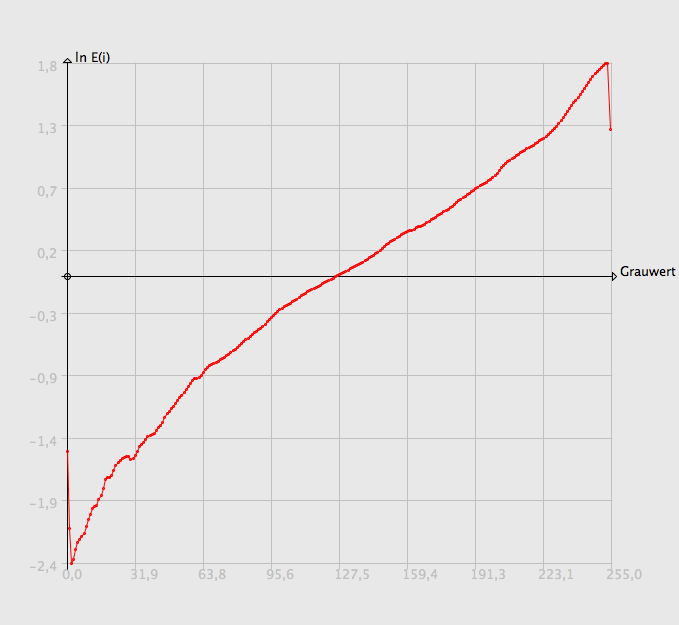
\includegraphics[width=3cm]{raum/g_ohne}}
            \end{overpic}
        };
        \spy on (1.4,-1.3) in node [left] at (9.5,0);
    \end{tikzpicture}
    \begin{tikzpicture}[spy using outlines={circle,red,magnification=3,size=4cm, connect spies}]
        \node {
            \begin{overpic}[width=0.5\textwidth]{robust/E_mit_robust_pepper}
                \put(-0,0){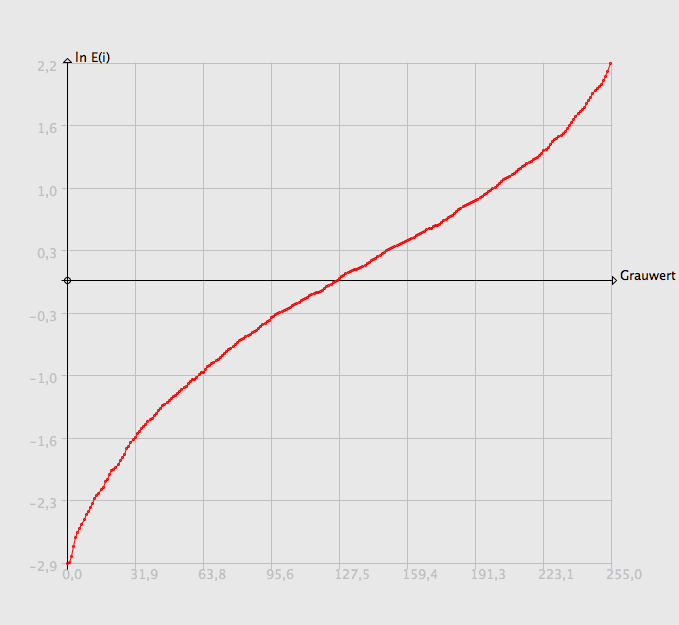
\includegraphics[width=3cm]{robust/g_mit_robust_pepper}}
            \end{overpic}
        };
        \spy on (1.4,-1.3) in node [left] at (9.5,0);
    \end{tikzpicture}
    
    \caption{\textit{Subquadratischen Bestrafungsfunktionen} --- \textbf{oben:} Standardverfahren mit \gls{SaltAndPepperNoise}, \textbf{unten:} Subquadratischer Bestrafungsterm $\varphi(s^2)=\sqrt{s^2+\epsilon^2}$ für $\b g$ und $\b E$ (das Rauschen ist quasi nicht mehr zu erkennen)}
    \label{fig:robust:2}
  \end{center}
\end{figure}


\begin{figure}
  \begin{center}
    \begin{tikzpicture}[spy using outlines={circle,red,magnification=3,size=4cm, connect spies}]
        \node {
            \begin{overpic}[width=0.5\textwidth]{robust/E_raum}
                \put(-0,0){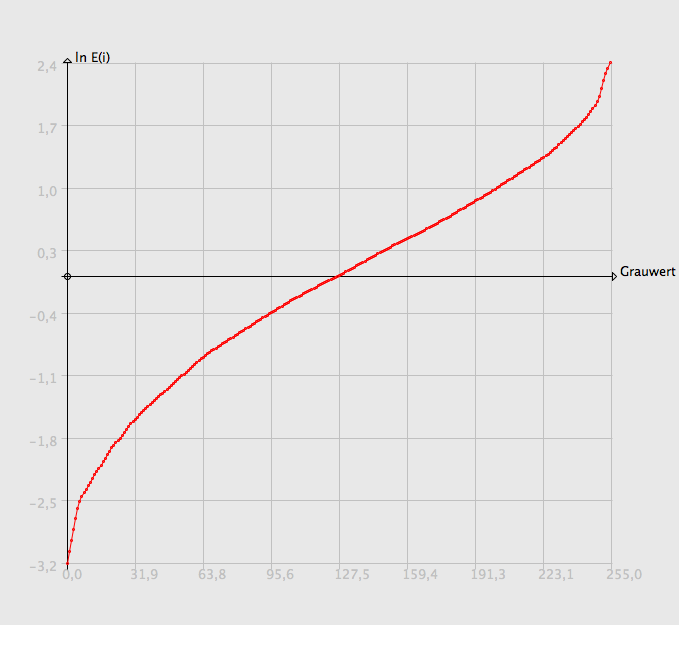
\includegraphics[width=3cm]{robust/g_raum}}
            \end{overpic}
        };
        \spy on (1.4,-1.3) in node [left] at (9.5,0);
    \end{tikzpicture}
        \begin{tikzpicture}[spy using outlines={circle,red,magnification=3,size=4cm, connect spies}]
        \node {
            \begin{overpic}[width=0.5\textwidth]{robust/E_raum_robust}
                \put(-0,0){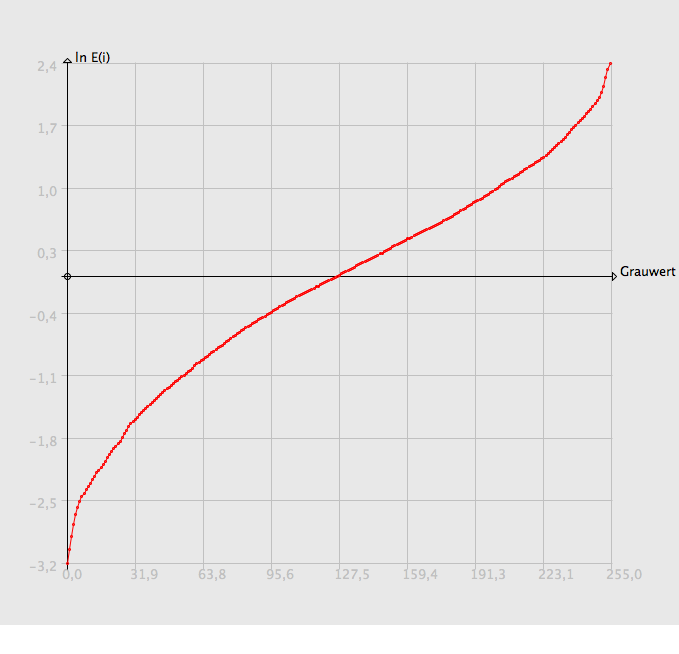
\includegraphics[width=3cm]{robust/g_raum_robust}}
            \end{overpic}
        };
        \spy on (1.4,-1.3) in node [left] at (9.5,0);
    \end{tikzpicture}

    \caption{\textit{Subquadratische Bestrafungsfunktionen (inkl. räumlicher Glattheitsterm und \gls{SaltAndPepperNoise}, $\alpha = 100$)} --- \textbf{oben:} Ohne subquadratische Bestrafungsfunktionen, \textbf{unten:} Mit subquadratischen Bestrafungsfunktionen}
    \label{fig:robust:kanten}
  \end{center}
\end{figure}

